\documentclass[sigconf]{acmart}

\setcopyright{none}
\settopmatter{printacmref=false,printfolios=true}
\renewcommand\footnotetextcopyrightpermission[1]{}
\pagestyle{plain}

\usepackage{booktabs}
\usepackage{graphicx}
\usepackage{amsmath}
\usepackage{siunitx}
\usepackage{enumitem}
\usepackage{algorithm}
\usepackage{algpseudocode}
\usepackage{pgfplots}
\usepgfplotslibrary{statistics}
\pgfplotsset{compat=1.18}

\title{Massively Parallel Multi-City Transit Schedule Analytics with MPI, MPI-I/O, and CUDA}

\author{Shimu Pan}
\affiliation{%
  \institution{Rensselaer Polytechnic Institute}
  \city{Troy}
  \state{New York}
  \country{USA}
}
\email{pans@rpi.edu}

\author{Tim Liakh}
\affiliation{%
  \institution{Rensselaer Polytechnic Institute}
  \city{Troy}
  \state{New York}
  \country{USA}
}
\email{replace-with-email@rpi.edu}

\author{Nikul Patel}
\affiliation{%
  \institution{Rensselaer Polytechnic Institute}
  \city{Troy}
  \state{New York}
  \country{USA}
}
\email{replace-with-email@rpi.edu}

\renewcommand{\shortauthors}{Pan, Liakh, and Patel}

\begin{document}

\begin{abstract}
Public transit agencies publish large General Transit Feed Specification (GTFS) datasets that encode routes, trips, calendars, and stop-level schedules for complex multi-modal systems. Although these feeds are standardized, they are still difficult to analyze at scale because useful system-level questions require combining many files, normalizing hundreds of thousands of schedule records, and aggregating spatiotemporal patterns across cities. This project presents a massively parallel pipeline for multi-city transit schedule analytics using MPI, MPI-I/O, and CUDA on the AiMOS supercomputer. Our pipeline downloads GTFS feeds from several major northeastern and midwestern transit providers, transforms them into a compact fixed-width binary representation, and performs collective parallel I/O using \texttt{MPI\_File\_read\_at\_all}. The workload is partitioned across MPI ranks, which exchange boundary records to preserve headway computations across partition edges and then reduce city-level statistics globally. Within each rank, a CUDA kernel accelerates bucketized departure analysis, trip-duration accumulation, and headway-regularity metrics on the GPU, while a CPU-only MPI backend provides a direct baseline for comparison. The resulting system measures peak-period service concentration, scheduled service intensity, bunching, wide-gap frequency, and route-level regularity proxies across providers. We design the implementation to support strong scaling, weak scaling, and explicit timing breakdowns for parallel I/O, communication, reduction, and computation, enabling an end-to-end study of hybrid distributed transit analytics that is both HPC-relevant and application-relevant.
\end{abstract}

\keywords{HPC, MPI, MPI-I/O, CUDA, GTFS, transit analytics, strong scaling, weak scaling}

\maketitle

\section{Introduction}
Public transit systems publish schedule data at a scale that is awkward for interactive analysis and expensive to normalize repeatedly. A single GTFS feed is a relational bundle of routes, trips, stop times, stops, calendars, and metadata. In practice, a multi-city study requires integrating many independent agency feeds, handling format quirks, deriving route-level and trip-level features, and then aggregating those features into interpretable system statistics. This is a natural problem for high-performance computing because the data volume is large, the preprocessing is expensive, and the final analytics require both local computation and global coordination.

This project targets that problem with a massively parallel system built around three ideas. First, we convert multi-file GTFS schedules into a fixed-width binary trip-record dataset that supports collective file access. Second, we use MPI and MPI-I/O to distribute that dataset across ranks, exchange boundary state, and reduce global aggregates. Third, we accelerate local analytics with CUDA so that each rank can use the GPU for bucketized schedule statistics and headway accumulation. The resulting workflow is not embarrassingly parallel because route headways cross partition boundaries, city-level statistics require collective reduction, and the input itself is read from a shared parallel file using MPI-I/O.

The application focus is \emph{scheduled service analysis}, not ridership analysis. Because the current pipeline uses static GTFS schedules rather than fare-card, passenger-count, or GTFS-Realtime delay data, the findings in this report concern service intensity, service mix, trip duration, and scheduled headway regularity. Those are still meaningful operational indicators, and they also produce a useful hybrid HPC workload with nontrivial communication and reduction behavior.

The main contributions of this project are:
\begin{itemize}[leftmargin=*]
  \item a GTFS preprocessing pipeline that converts heterogeneous public feeds into one compact binary dataset suitable for collective MPI-I/O;
  \item a distributed analytics engine that combines MPI partitioning, boundary exchange, reduction, and CUDA local processing;
  \item a provider-level transit analysis across five major agencies using real GTFS schedule data; and
  \item an experimental design for strong scaling, weak scaling, and CPU-versus-GPU comparison on AiMOS.
\end{itemize}

\section{Related Work}
GTFS has become a standard substrate for transit network analysis. The official GTFS schedule and GTFS-Realtime specifications define the semantics and field structure for static and live transit data~\cite{gtfs_schedule_ref,gtfs_realtime_ref,gtfs_overview}. Those specifications make ecosystem-wide tooling possible, but they do not remove the underlying cost of integrating schedule, calendar, and stop-time files into analytical features.

Several prior works demonstrate the analytical value of GTFS. Fayyaz et al.~\cite{fayyaz2017gtfs} developed an efficient GTFS-enabled algorithm for dynamic transit accessibility analysis. Fortin et al.~\cite{fortin2016gtfs} used GTFS data to build graph-oriented transit network indicators, while Guthrie et al.~\cite{guthrie2017accessibility} used GTFS for accessibility scenario analysis in sketch planning. Pereira et al.~\cite{pereira2021r5r} introduced a practical multimodal routing framework that relies on GTFS-style network data and supports accessibility-oriented queries at scale.

Recent work has pushed transit analysis toward richer operational and interactive settings. Devunuri and Lehe~\cite{devunuri2025transitgpt} showed that GTFS datasets can support flexible analytical querying through large language model interfaces. Javanmard et al.~\cite{javanmard2025realtime} and Zhou et al.~\cite{zhou2024latency} highlight the growing importance of GTFS-Realtime for uncertainty-aware accessibility and operational decision support. These studies reinforce the need for scalable data-processing infrastructure that can handle multiple feeds and repeated analytics efficiently.

On the HPC side, our implementation rests on standard distributed and accelerator programming models. The MPI 4.1 standard provides the collective communication and MPI-I/O interfaces used by our code~\cite{mpi41}. Thakur et al.~\cite{thakur1999romio} describe the role of collective I/O and data sieving in ROMIO, which directly motivates our use of \texttt{MPI\_File\_read\_at\_all} over a shared binary dataset. For GPU acceleration, our implementation follows the CUDA programming model described by Nickolls et al.~\cite{nickolls2008cuda} and NVIDIA’s programming guide~\cite{cuda_guide}. The contribution here is not a new HPC runtime in isolation, but the application of these models to a transit-schedule workload whose irregularity, shared input, and provider-wide aggregation make it a meaningful massively parallel case study.

\section{Dataset and Problem Formulation}
\subsection{Provider Set}
The current dataset covers five provider groups assembled from publicly accessible GTFS schedule feeds:
\begin{itemize}[leftmargin=*]
  \item MTA (New York): subway, commuter rail, and several bus subfeeds,
  \item CTA (Chicago),
  \item MBTA (Boston),
  \item NJ Transit, and
  \item SEPTA (Philadelphia).
\end{itemize}

The preprocessing stage currently produces a consolidated binary dataset of \num{576229} trip records, each exactly 48 bytes. Table~\ref{tab:dataset} summarizes the resulting provider-level record counts and route counts derived during preprocessing.

\begin{table}[t]
  \centering
  \caption{Local GTFS dataset summary after preprocessing.}
  \label{tab:dataset}
  \begin{tabular}{lrr}
    \toprule
    \textbf{Provider} & \textbf{Trip Records} & \textbf{Unique Routes} \\
    \midrule
    MTA & 287,347 & 392 \\
    CTA & 94,496 & 131 \\
    MBTA & 121,506 & 374 \\
    NJ Transit & 36,483 & 279 \\
    SEPTA & 36,397 & 184 \\
    \midrule
    Total & 576,229 & 1,360 \\
    \bottomrule
  \end{tabular}
\end{table}

\subsection{Trip-Record Representation}
The preprocessing stage converts each GTFS trip into a fixed-width record:
\begin{quote}
\small\ttfamily
(city\_id, feed\_id, route\_type, route\_hash, service\_mask,\\
direction\_id, start\_secs, end\_secs, duration\_secs, stop\_count,\\
trip\_hash, reserved)
\end{quote}
This representation is intentionally compact. It avoids expensive string parsing during parallel execution and allows the MPI layer to partition input by record count rather than by text-file boundaries.

Records are sorted by:
\begin{quote}
\small\ttfamily
(city\_id, route\_hash, direction\_id, start\_secs, trip\_hash)
\end{quote}
That sort order is critical because the route-headway computation depends on adjacent records within each city, route, and direction.

\subsection{Analytical Questions}
This report focuses on two types of questions:
\begin{enumerate}[leftmargin=*]
  \item \textbf{HPC questions}: How does the hybrid MPI+CUDA implementation behave under strong scaling, weak scaling, and CPU-versus-GPU comparison? How much time is spent on file I/O, communication, reduction, and compute?
  \item \textbf{Transit questions}: How do providers differ in peak/off-peak concentration, scheduled headway structure, hourly service profile, and mode composition?
\end{enumerate}

The second class of questions is not only useful for the application; it also justifies the first. The point of accelerating the workload is to make these provider-level insights practical at larger scale and over richer data.

\section{Parallel Algorithm - CUDA and MPI}
\subsection{Pipeline Overview}
Figure~\ref{fig:pipeline} shows the end-to-end workflow.

\begin{figure}[t]
  \centering
  \fbox{\parbox{0.95\columnwidth}{
    \textbf{Pipeline:} GTFS download $\rightarrow$ preprocessing into fixed-width binary records $\rightarrow$ collective MPI-I/O read $\rightarrow$ rank-boundary exchange $\rightarrow$ CPU or CUDA local analytics $\rightarrow$ MPI reduction $\rightarrow$ provider-level summaries and performance reports.
  }}
  \caption{High-level workflow implemented in this project.}
  \label{fig:pipeline}
\end{figure}

\subsection{Preprocessing}
The preprocessing stage is implemented in Python. It reads \texttt{routes.txt}, \texttt{trips.txt}, \texttt{stop\_times.txt}, and calendar metadata and then derives one record per trip. During implementation, several real-world GTFS packaging differences had to be handled explicitly:
\begin{itemize}[leftmargin=*]
  \item some feeds include \texttt{calendar\_dates.txt} but no \texttt{calendar.txt};
  \item some providers package multiple nested GTFS archives inside one top-level zip; and
  \item route-type values are not always limited to the canonical small GTFS set, so extended values must later be normalized for reporting.
\end{itemize}
These details matter because a realistic system has to accommodate provider-specific packaging, not just idealized feeds.

\subsection{MPI-I/O and Partitioning}
At runtime, the analyzer opens the binary dataset collectively with \texttt{MPI\_File\_open}, obtains the file size, converts it to a record count, and partitions the record range across ranks. Each rank then issues a collective \texttt{MPI\_File\_read\_at\_all} to fetch its contiguous record block.

This design avoids the serial bottleneck of a rank-0 reader followed by a broadcast or scatter of the data. It also lets the input path itself become part of the performance study, which is required by the project rubric whenever I/O is a major component.

\subsection{Boundary Exchange}
The workload is not embarrassingly parallel because route headways depend on neighboring records across partition boundaries. If one rank ends with trip $t_i$ and the next rank begins with trip $t_{i+1}$ on the same route-direction pair, the headway between them must still be counted. The implementation therefore performs a boundary exchange with \texttt{MPI\_Sendrecv} so that each rank can compare its first local trip to the previous rank’s last trip.

\subsection{CPU and CUDA Backends}
The local analytics stage supports two interchangeable backends:
\begin{itemize}[leftmargin=*]
  \item \textbf{CPU backend}: MPI-distributed host-side accumulation for all statistics;
  \item \textbf{CUDA backend}: GPU-accelerated local analysis within each rank.
\end{itemize}

The CUDA path uses the rank’s node-local communicator to select a GPU deterministically and then copies the local record partition to device memory. A CUDA kernel computes departures per time bucket, route-type counts, trip-duration sums, stop-count sums, and headway-related aggregates.

\begin{algorithm}[t]
\caption{Distributed Transit Analytics}
\label{alg:analysis}
\begin{algorithmic}[1]
\Require Sorted binary trip-record dataset; backend $\in \{\texttt{cpu}, \texttt{cuda}\}$
\State Open dataset collectively with MPI-I/O
\State Partition records across ranks
\State Read local block with \texttt{MPI\_File\_read\_at\_all}
\State Exchange one boundary record with neighboring rank
\If{backend = \texttt{cuda}}
  \State Copy local block to GPU
  \State Launch CUDA kernel to accumulate local statistics
\Else
  \State Accumulate local statistics on CPU
\EndIf
\State Reduce local arrays and sums to rank 0
\State Emit timing, provider summaries, and optional CSV reports
\end{algorithmic}
\end{algorithm}

\subsection{Global Reduction}
Each rank computes local counts, sums, and squared sums. Rank~0 receives the global totals with \texttt{MPI\_Reduce}, then derives:
\begin{itemize}[leftmargin=*]
  \item hourly departure profiles,
  \item peak/off-peak ratios,
  \item route-type counts,
  \item mean and coefficient of variation of headways,
  \item bunching and wide-gap rates, and
  \item trip-duration summaries.
\end{itemize}
Because the local arrays must be combined to produce provider-level outputs, the analysis necessarily includes a collective aggregation stage.

\section{Experimental Methodology}
All cluster experiments target AiMOS POWER9 nodes with NVIDIA V100 GPUs and use the module stack
\begin{quote}
\texttt{module load xl\_r spectrum-mpi cuda}
\end{quote}
as described in the course materials. The build process compiles the MPI logic with \texttt{mpicc} and the CUDA logic with \texttt{nvcc}, then links the resulting objects into a single executable.

The planned performance study follows the assignment requirements:
\begin{enumerate}[leftmargin=*]
  \item \textbf{Strong scaling}: fix the total record count and increase the rank count.
  \item \textbf{Weak scaling}: fix the records per rank and grow the total dataset proportionally.
  \item \textbf{CPU-only MPI vs.\ hybrid MPI+CUDA}: compare the two backends directly.
\end{enumerate}

Each run reports:
\begin{itemize}[leftmargin=*]
  \item MPI-I/O time,
  \item boundary-exchange time,
  \item local compute time,
  \item reduction time, and
  \item total runtime.
\end{itemize}
This breakdown is essential because the goal is not just to show speedup, but to explain whether bottlenecks come from shared-file access, communication, or actual computation.

\begin{table}[t]
  \centering
  \caption{Experiment matrix used for the AiMOS timing study.}
  \label{tab:expmatrix}
  \begin{tabular}{lll}
    \toprule
    \textbf{Study} & \textbf{Ranks} & \textbf{Requested Records} \\
    \midrule
    Strong scaling & 2, 4, 8, 16 & 400,000 fixed \\
    Weak scaling & 2, 4, 8, 16 & 150,000 per rank \\
    \bottomrule
  \end{tabular}
\end{table}

At this point, both the provider-analysis workflow and the AiMOS timing workflow are producing reportable outputs. The provider-analysis figures come from the local GTFS-derived binary dataset, while the timing figures come from the successful AiMOS experiment sweeps recorded in \texttt{experiment\_results.csv}. In the weak-scaling experiments, requested record counts beyond the local dataset size are clamped by the available input, so the largest weak-scaling runs ultimately operate on the full 576,229-record dataset.

\section{Transit Provider Findings}
\subsection{Peak vs.\ Off-Peak Concentration}
Figure~\ref{fig:peakoffpeak} compares the ratio of peak-period trip starts to off-peak trip starts for each provider. We define peak as 7--10 AM and 4--7 PM. NJ Transit shows the largest concentration of service in those windows, with a peak/off-peak ratio of approximately 0.607. The other agencies cluster more tightly around 0.50--0.55. This suggests that NJ Transit is more commuter-peaked, while the urban systems provide relatively more all-day service.

\begin{figure}[t]
  \centering
  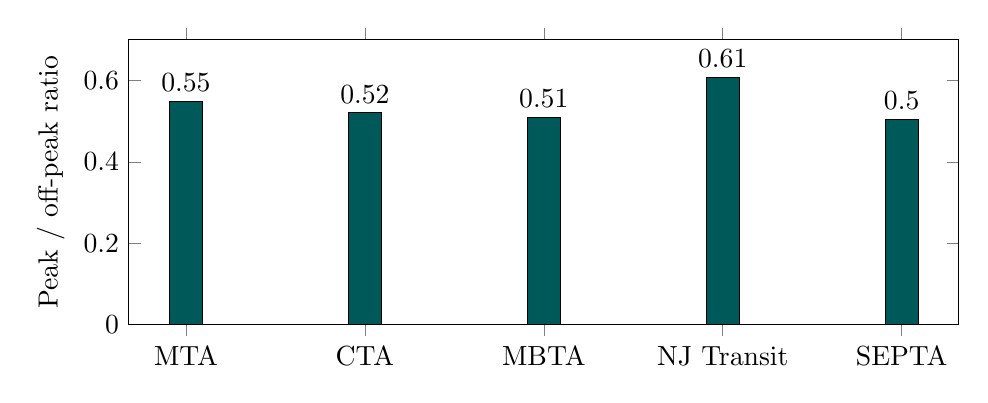
\begin{tikzpicture}
  \begin{axis}[
    ybar,
    width=\columnwidth,
    height=5.2cm,
    bar width=12pt,
    symbolic x coords={MTA,CTA,MBTA,NJ Transit,SEPTA},
    xtick=data,
    ylabel={Peak / off-peak ratio},
    ymin=0,
    ymax=0.7,
    nodes near coords,
    nodes near coords align={vertical},
    enlarge x limits=0.08
  ]
  \addplot[fill=teal!70!black] coordinates {
    (MTA,0.5482)
    (CTA,0.5205)
    (MBTA,0.5094)
    (NJ Transit,0.6068)
    (SEPTA,0.5038)
  };
  \end{axis}
  \end{tikzpicture}
  \caption{Peak/off-peak service ratio by provider, computed from local GTFS trip-start counts.}
  \label{fig:peakoffpeak}
\end{figure}

\subsection{Hourly Service Profile}
Figure~\ref{fig:hourlyprofile} shows the hourly trip-start counts for each provider. MTA dominates in absolute service volume throughout the day, which is expected given the number of subfeeds included in the New York provider grouping. The shape of the curves is still informative: all providers show strong morning growth into the 6--8 AM window, a midday plateau, and then a smaller afternoon bump before evening decline. CTA displays the flattest daytime profile among the urban agencies, while NJ Transit drops off more sharply outside peak commuter periods.

\begin{figure*}[t]
  \centering
  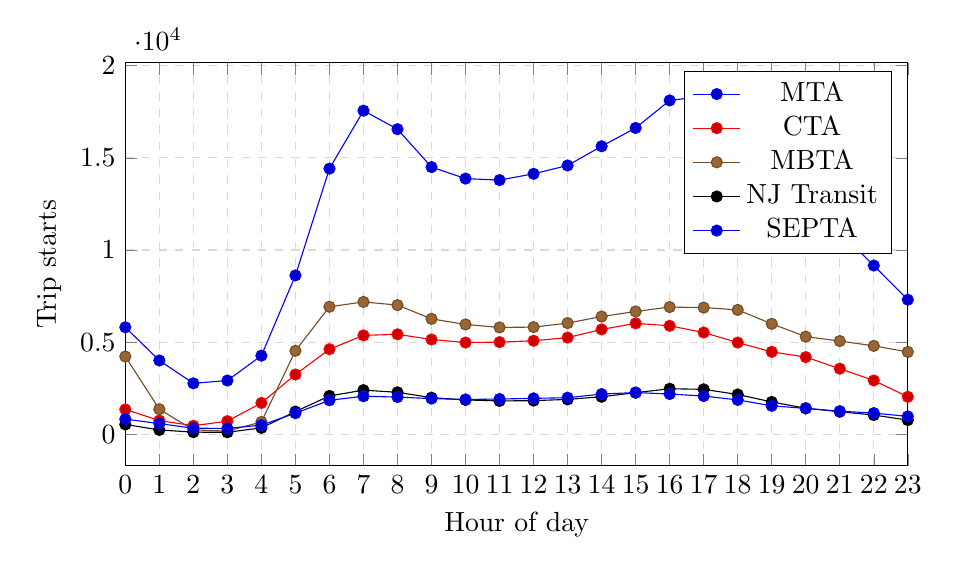
\begin{tikzpicture}
  \begin{axis}[
    width=0.95\textwidth,
    height=6.7cm,
    xlabel={Hour of day},
    ylabel={Trip starts},
    xmin=0, xmax=23,
    xtick={0,1,2,3,4,5,6,7,8,9,10,11,12,13,14,15,16,17,18,19,20,21,22,23},
    grid=both,
    grid style={dashed,gray!30},
    legend style={at={(0.98,0.98)},anchor=north east}
  ]
  \addplot+[mark=*] coordinates {
    (0,5809) (1,4011) (2,2772) (3,2925) (4,4274) (5,8623) (6,14411) (7,17553)
    (8,16550) (9,14495) (10,13871) (11,13790) (12,14131) (13,14582) (14,15624)
    (15,16617) (16,18109) (17,18326) (18,16714) (19,14352) (20,12362) (21,10982)
    (22,9158) (23,7306)
  };
  \addlegendentry{MTA}
  \addplot+[mark=*] coordinates {
    (0,1357) (1,756) (2,472) (3,723) (4,1711) (5,3250) (6,4622) (7,5371)
    (8,5429) (9,5149) (10,4983) (11,5006) (12,5081) (13,5252) (14,5696)
    (15,6026) (16,5891) (17,5527) (18,4983) (19,4480) (20,4194) (21,3567)
    (22,2928) (23,2042)
  };
  \addlegendentry{CTA}
  \addplot+[mark=*] coordinates {
    (0,4228) (1,1368) (2,248) (3,183) (4,681) (5,4536) (6,6923) (7,7185)
    (8,7013) (9,6267) (10,5965) (11,5803) (12,5820) (13,6037) (14,6394)
    (15,6668) (16,6907) (17,6878) (18,6754) (19,5999) (20,5305) (21,5065)
    (22,4804) (23,4475)
  };
  \addlegendentry{MBTA}
  \addplot+[mark=*] coordinates {
    (0,542) (1,246) (2,125) (3,119) (4,358) (5,1239) (6,2090) (7,2403)
    (8,2286) (9,1995) (10,1872) (11,1819) (12,1834) (13,1901) (14,2044)
    (15,2266) (16,2479) (17,2447) (18,2168) (19,1763) (20,1422) (21,1232)
    (22,1054) (23,779)
  };
  \addlegendentry{NJ Transit}
  \addplot+[mark=*] coordinates {
    (0,831) (1,588) (2,338) (3,330) (4,506) (5,1154) (6,1853) (7,2073)
    (8,2027) (9,1945) (10,1898) (11,1921) (12,1958) (13,1993) (14,2189)
    (15,2273) (16,2192) (17,2084) (18,1873) (19,1554) (20,1415) (21,1263)
    (22,1159) (23,980)
  };
  \addlegendentry{SEPTA}
  \end{axis}
  \end{tikzpicture}
  \caption{Hourly scheduled trip starts by provider.}
  \label{fig:hourlyprofile}
\end{figure*}

\subsection{Service Span and Overnight Coverage}
Hourly volume alone does not show how long each system remains active across the service day. Figure~\ref{fig:servicespan} compares the first scheduled departure and last scheduled arrival observed in each provider’s GTFS records, measured in service-day hours rather than clock hours so that overnight trips beyond midnight remain visible. MBTA and NJ Transit extend furthest into the late-night or early-morning tail, while CTA’s scheduled service span ends somewhat earlier. MTA begins exactly at the start of the service day and extends to about hour 28.8, reflecting overnight service that continues well beyond midnight. This is a useful complement to the hourly profile because two systems may have similar daytime totals but very different late-night coverage.

\begin{figure}[t]
  \centering
  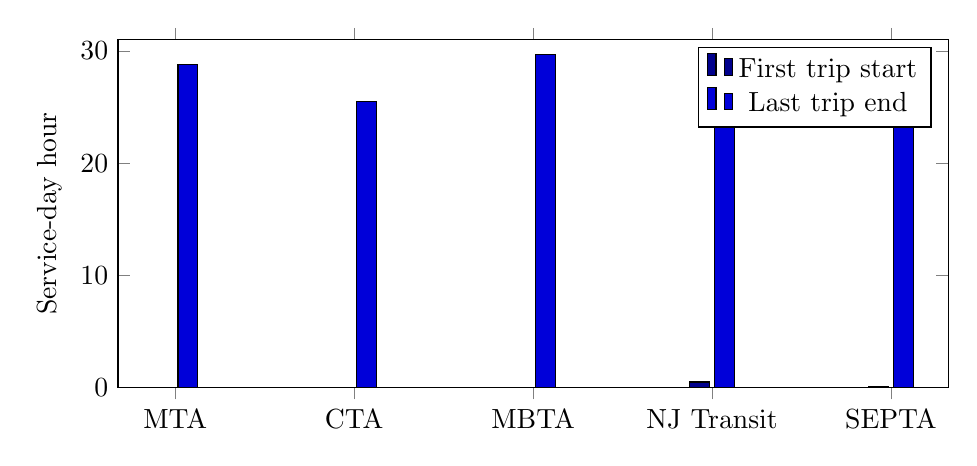
\begin{tikzpicture}
  \begin{axis}[
    ybar,
    width=\columnwidth,
    height=6cm,
    bar width=7pt,
    symbolic x coords={MTA,CTA,MBTA,NJ Transit,SEPTA},
    xtick=data,
    ylabel={Service-day hour},
    ymin=0,
    ymax=31,
    enlarge x limits=0.08,
    legend style={at={(0.98,0.98)},anchor=north east}
  ]
  \addplot[fill=blue!55!black] coordinates {
    (MTA,0.00) (CTA,0.00) (MBTA,0.00) (NJ Transit,0.50) (SEPTA,0.10)
  };
  \addlegendentry{First trip start}
  \addplot[fill=blue!85!black] coordinates {
    (MTA,28.80) (CTA,25.50) (MBTA,29.72) (NJ Transit,29.17) (SEPTA,27.90)
  };
  \addlegendentry{Last trip end}
  \end{axis}
  \end{tikzpicture}
  \caption{Scheduled service span by provider, measured in service-day hours so that overnight trips remain visible.}
  \label{fig:servicespan}
\end{figure}

\subsection{Headway Distribution}
Headway statistics reveal stronger differences than the peak/off-peak ratio alone. Figure~\ref{fig:headwaybox} summarizes the distribution of mean route headways by provider using quartiles computed over route-direction groups. CTA and MTA show the smallest median route headways, about 3.30 and 4.39 minutes respectively, reflecting dense urban transit service. MBTA’s median is higher, about 5.86 minutes, while SEPTA and especially NJ Transit show much wider and larger headways. NJ Transit’s median route headway is approximately 20.53 minutes, consistent with a service mix oriented toward commuter rail and less frequent regional operation.

\begin{figure}[t]
  \centering
  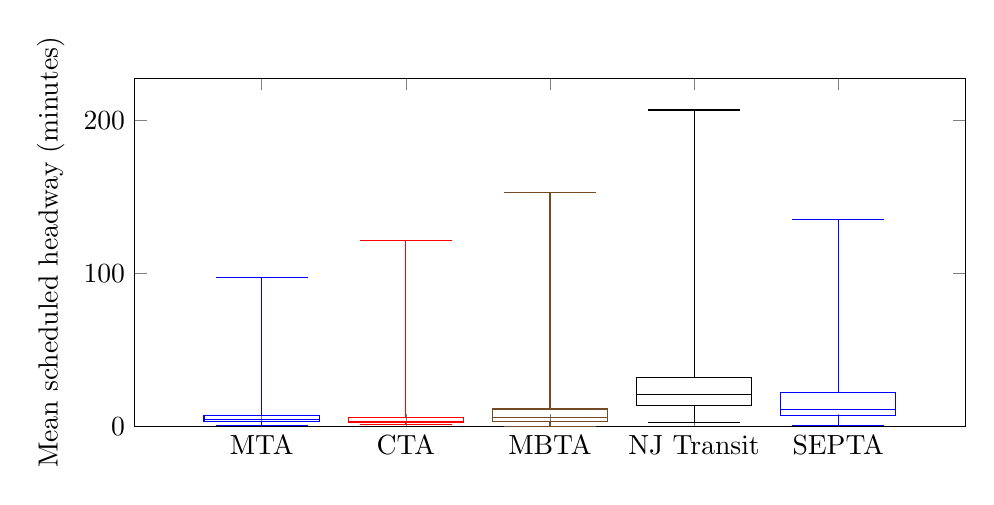
\begin{tikzpicture}
  \begin{axis}[
    width=\columnwidth,
    height=6cm,
    ylabel={Mean scheduled headway (minutes)},
    xtick={1,2,3,4,5},
    xticklabels={MTA,CTA,MBTA,NJ Transit,SEPTA},
    ymin=0,
    boxplot/draw direction=y
  ]
  \addplot+[
    boxplot prepared={
      lower whisker=0.3488, lower quartile=3.1900, median=4.3944, upper quartile=6.7836, upper whisker=97.2222
    },
  ] coordinates {};
  \addplot+[
    boxplot prepared={
      lower whisker=1.2207, lower quartile=2.5088, median=3.3048, upper quartile=5.7627, upper whisker=121.1111
    },
  ] coordinates {};
  \addplot+[
    boxplot prepared={
      lower whisker=0.0, lower quartile=3.1633, median=5.8633, upper quartile=11.2450, upper whisker=152.8571
    },
  ] coordinates {};
  \addplot+[
    boxplot prepared={
      lower whisker=2.5569, lower quartile=13.3784, median=20.5263, upper quartile=31.9429, upper whisker=206.6667
    },
  ] coordinates {};
  \addplot+[
    boxplot prepared={
      lower whisker=0.5, lower quartile=6.8827, median=10.8235, upper quartile=22.0, upper whisker=135.0
    },
  ] coordinates {};
  \end{axis}
  \end{tikzpicture}
  \caption{Distribution of route-level mean scheduled headways by provider.}
  \label{fig:headwaybox}
\end{figure}

\subsection{Trip Duration Distribution}
Figure~\ref{fig:durationbox} compares the scheduled trip-duration distributions derived from GTFS start and end times. This metric helps separate systems with dense, short urban trips from systems with longer regional or commuter-oriented runs. MBTA has the lowest median scheduled trip duration at roughly 29 minutes, while MTA, CTA, and NJ Transit cluster near 50 minutes. NJ Transit also has the broadest upper tail, reaching nearly 297 minutes in the maximum observed scheduled duration, which is consistent with longer-distance commuter services. SEPTA sits between the dense urban systems and the regional systems with a median scheduled duration of about 39 minutes.

\begin{figure}[t]
  \centering
  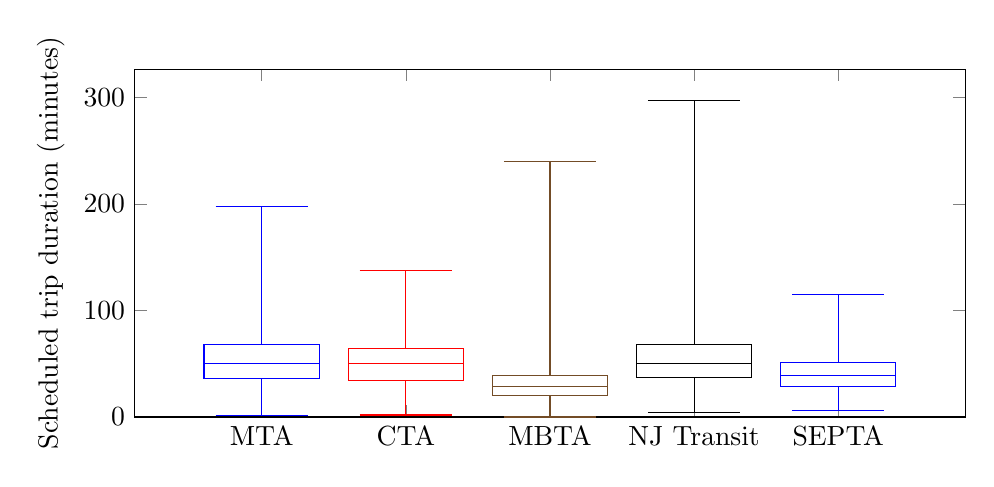
\begin{tikzpicture}
  \begin{axis}[
    width=\columnwidth,
    height=6cm,
    ylabel={Scheduled trip duration (minutes)},
    xtick={1,2,3,4,5},
    xticklabels={MTA,CTA,MBTA,NJ Transit,SEPTA},
    ymin=0,
    boxplot/draw direction=y
  ]
  \addplot+[
    boxplot prepared={
      lower whisker=1.5, lower quartile=36.0, median=50.0, upper quartile=68.0, upper whisker=198.0
    },
  ] coordinates {};
  \addplot+[
    boxplot prepared={
      lower whisker=1.93, lower quartile=34.0, median=50.5, upper quartile=64.0, upper whisker=138.0
    },
  ] coordinates {};
  \addplot+[
    boxplot prepared={
      lower whisker=0.0, lower quartile=20.0, median=29.0, upper quartile=39.0, upper whisker=240.0
    },
  ] coordinates {};
  \addplot+[
    boxplot prepared={
      lower whisker=4.0, lower quartile=37.0, median=50.0, upper quartile=68.0, upper whisker=297.0
    },
  ] coordinates {};
  \addplot+[
    boxplot prepared={
      lower whisker=6.0, lower quartile=29.0, median=39.0, upper quartile=51.0, upper whisker=115.0
    },
  ] coordinates {};
  \end{axis}
  \end{tikzpicture}
  \caption{Distribution of scheduled trip durations by provider.}
  \label{fig:durationbox}
\end{figure}

\subsection{Mode Composition}
Figure~\ref{fig:modecomposition} compares provider mode composition using normalized GTFS route types. Bus routes dominate every provider group in absolute count, but the secondary composition varies. MTA includes a meaningful amount of subway and commuter rail service; MBTA shows the richest mode mix, including subway, rail, tram, and ferry; SEPTA also has a more visibly multimodal profile than CTA. These mode differences help explain the headway distributions above.

\begin{figure}[t]
  \centering
  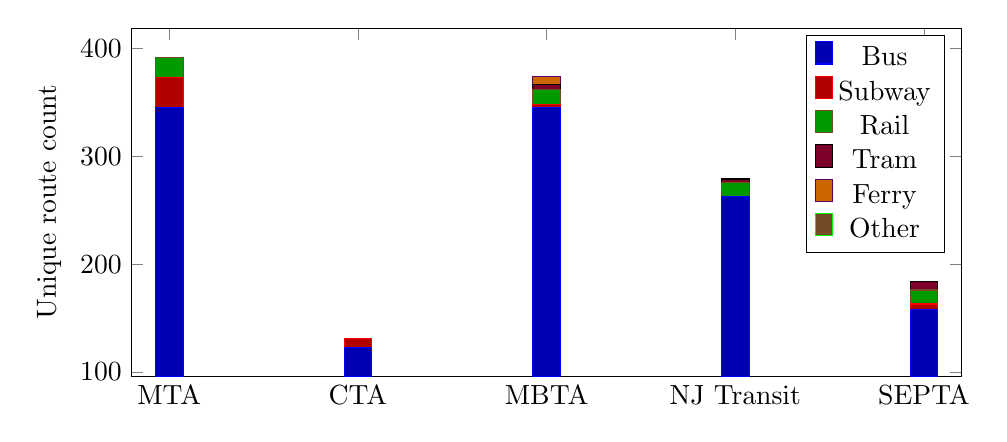
\begin{tikzpicture}
  \begin{axis}[
    ybar stacked,
    width=\columnwidth,
    height=6cm,
    bar width=10pt,
    symbolic x coords={MTA,CTA,MBTA,NJ Transit,SEPTA},
    xtick=data,
    ylabel={Unique route count},
    enlarge x limits=0.05,
    legend style={at={(0.98,0.98)},anchor=north east}
  ]
  \addplot+[fill=blue!70!black] coordinates {(MTA,345) (CTA,123) (MBTA,345) (NJ Transit,263) (SEPTA,158)};
  \addlegendentry{Bus}
  \addplot+[fill=red!70!black] coordinates {(MTA,28) (CTA,8) (MBTA,3) (NJ Transit,0) (SEPTA,5)};
  \addlegendentry{Subway}
  \addplot+[fill=green!60!black] coordinates {(MTA,19) (CTA,0) (MBTA,14) (NJ Transit,13) (SEPTA,13)};
  \addlegendentry{Rail}
  \addplot+[fill=purple!65!black] coordinates {(MTA,0) (CTA,0) (MBTA,5) (NJ Transit,3) (SEPTA,8)};
  \addlegendentry{Tram}
  \addplot+[fill=orange!80!black] coordinates {(MTA,0) (CTA,0) (MBTA,7) (NJ Transit,0) (SEPTA,0)};
  \addlegendentry{Ferry}
  \addplot+[fill=brown!60!black] coordinates {(MTA,0) (CTA,0) (MBTA,0) (NJ Transit,0) (SEPTA,0)};
  \addlegendentry{Other}
  \end{axis}
  \end{tikzpicture}
  \caption{Provider mode composition after GTFS route-type normalization.}
  \label{fig:modecomposition}
\end{figure}

\subsection{Route Intensity}
Absolute route counts can be misleading because large systems may spread service thinly across many routes or concentrate many trips on fewer corridors. Figure~\ref{fig:routeintensity} therefore normalizes total trip starts by unique route count. MTA and CTA both exceed 720 scheduled trip starts per unique route in the local dataset snapshot, while MBTA drops to about 325 and the regional systems are lower still. NJ Transit is the least intensive by this measure, at roughly 131 scheduled trip starts per unique route. This graph is useful because it combines network breadth with schedule density in one number and helps explain why urban systems can have short median headways even when total route counts are not dramatically larger.

\begin{figure}[t]
  \centering
  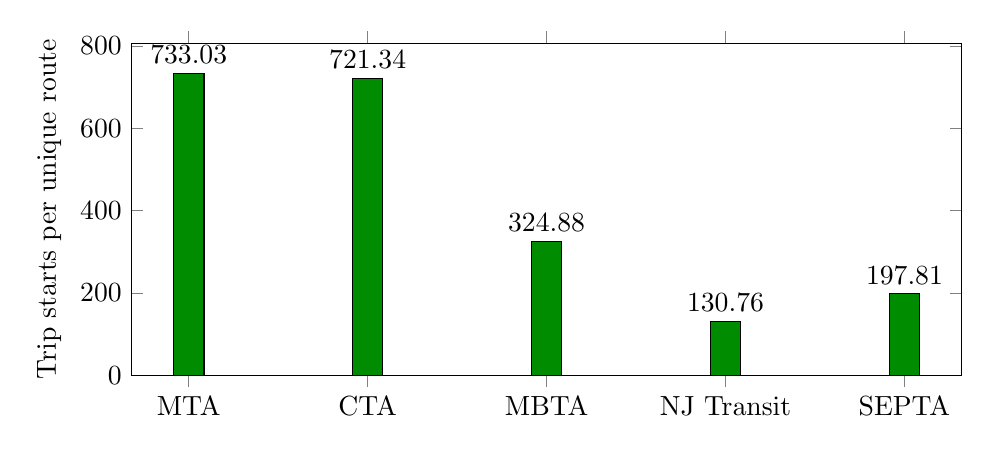
\begin{tikzpicture}
  \begin{axis}[
    ybar,
    width=\columnwidth,
    height=5.8cm,
    bar width=11pt,
    symbolic x coords={MTA,CTA,MBTA,NJ Transit,SEPTA},
    xtick=data,
    ylabel={Trip starts per unique route},
    ymin=0,
    enlarge x limits=0.08,
    nodes near coords,
    nodes near coords align={vertical}
  ]
  \addplot[fill=green!55!black] coordinates {
    (MTA,733.03)
    (CTA,721.34)
    (MBTA,324.88)
    (NJ Transit,130.76)
    (SEPTA,197.81)
  };
  \end{axis}
  \end{tikzpicture}
  \caption{Scheduled route intensity by provider, defined as trip starts divided by unique route count.}
  \label{fig:routeintensity}
\end{figure}

\subsection{Headway Irregularity Proxies}
The parallel analyzer also emits schedule-regularity proxies such as bunch-rate and wide-gap-rate summaries. These are not realtime reliability measures; instead, they describe how frequently the scheduled headways in each city fall below or above fixed threshold bands. Figure~\ref{fig:irregularity} shows a useful split between dense urban systems and regional systems. MTA, CTA, and MBTA all show high bunch-rate proxies, which is expected because many route-direction groups operate on short headways where successive departures often fall into a ``very short'' bucket. NJ Transit and SEPTA, by contrast, show much larger wide-gap rates, reflecting the lower-frequency structure already visible in the headway distribution figure. This plot is worth including because it comes from the actual MPI/CUDA analytics engine rather than only from the preprocessing pass.

\begin{figure}[t]
  \centering
  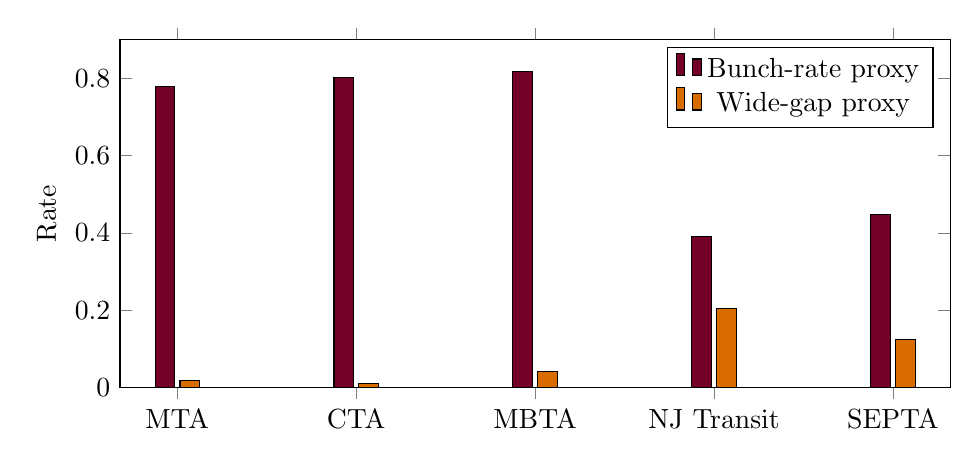
\begin{tikzpicture}
  \begin{axis}[
    ybar,
    width=\columnwidth,
    height=6cm,
    bar width=7pt,
    symbolic x coords={MTA,CTA,MBTA,NJ Transit,SEPTA},
    xtick=data,
    ylabel={Rate},
    ymin=0,
    ymax=0.9,
    enlarge x limits=0.08,
    legend style={at={(0.98,0.98)},anchor=north east}
  ]
  \addplot[fill=purple!60!black] coordinates {
    (MTA,0.7790) (CTA,0.8013) (MBTA,0.8189) (NJ Transit,0.3921) (SEPTA,0.4470)
  };
  \addlegendentry{Bunch-rate proxy}
  \addplot[fill=orange!85!black] coordinates {
    (MTA,0.0175) (CTA,0.0103) (MBTA,0.0418) (NJ Transit,0.2043) (SEPTA,0.1251)
  };
  \addlegendentry{Wide-gap proxy}
  \end{axis}
  \end{tikzpicture}
  \caption{Schedule irregularity proxies emitted by the parallel analyzer.}
  \label{fig:irregularity}
\end{figure}

\subsection{Provider Summary}
Table~\ref{tab:providersummary} collects the main provider-side metrics used in this report. The table is useful both as an application result and as a sanity check that the preprocessing stage is capturing plausible system-scale patterns.

\begin{table*}[t]
  \centering
  \caption{Provider-level schedule summary derived from the local binary dataset.}
  \label{tab:providersummary}
  \begin{tabular}{lrrrrrrrr}
    \toprule
    \textbf{Provider} & \textbf{Trip Starts} & \textbf{Peak/Off-Peak} & \textbf{Median Headway (min)} & \textbf{Avg Duration (min)} & \textbf{Trips/Route} & \textbf{Service Span (hr)} & \textbf{Unique Routes} & \textbf{Dominant Mode} \\
    \midrule
    MTA & 287,347 & 0.548 & 4.39 & 53.21 & 733.03 & 0.00--28.80 & 392 & Bus \\
    CTA & 94,496 & 0.521 & 3.30 & 50.69 & 721.34 & 0.00--25.50 & 131 & Bus \\
    MBTA & 121,506 & 0.509 & 5.86 & 30.88 & 324.88 & 0.00--29.72 & 374 & Bus \\
    NJ Transit & 36,483 & 0.607 & 20.53 & 55.60 & 130.76 & 0.50--29.17 & 279 & Bus \\
    SEPTA & 36,397 & 0.504 & 10.82 & 40.62 & 197.81 & 0.10--27.90 & 184 & Bus \\
    \bottomrule
  \end{tabular}
\end{table*}

\section{Strong Scaling Parallel Performance}
\label{sec:strong-scaling}
The figures in this section were generated from the AiMOS output stored in \texttt{experiment\_results.csv}. The observed performance story is more nuanced than the original expectation of a straightforward GPU win: the local CUDA compute kernel is fast, but the end-to-end wall-clock time of the GPU path is dominated by GPU setup and runtime overhead that is not present in the CPU-only MPI baseline. That distinction is important because the assignment asks for total performance analysis, not just kernel timings.

\begin{figure}[t]
  \centering
  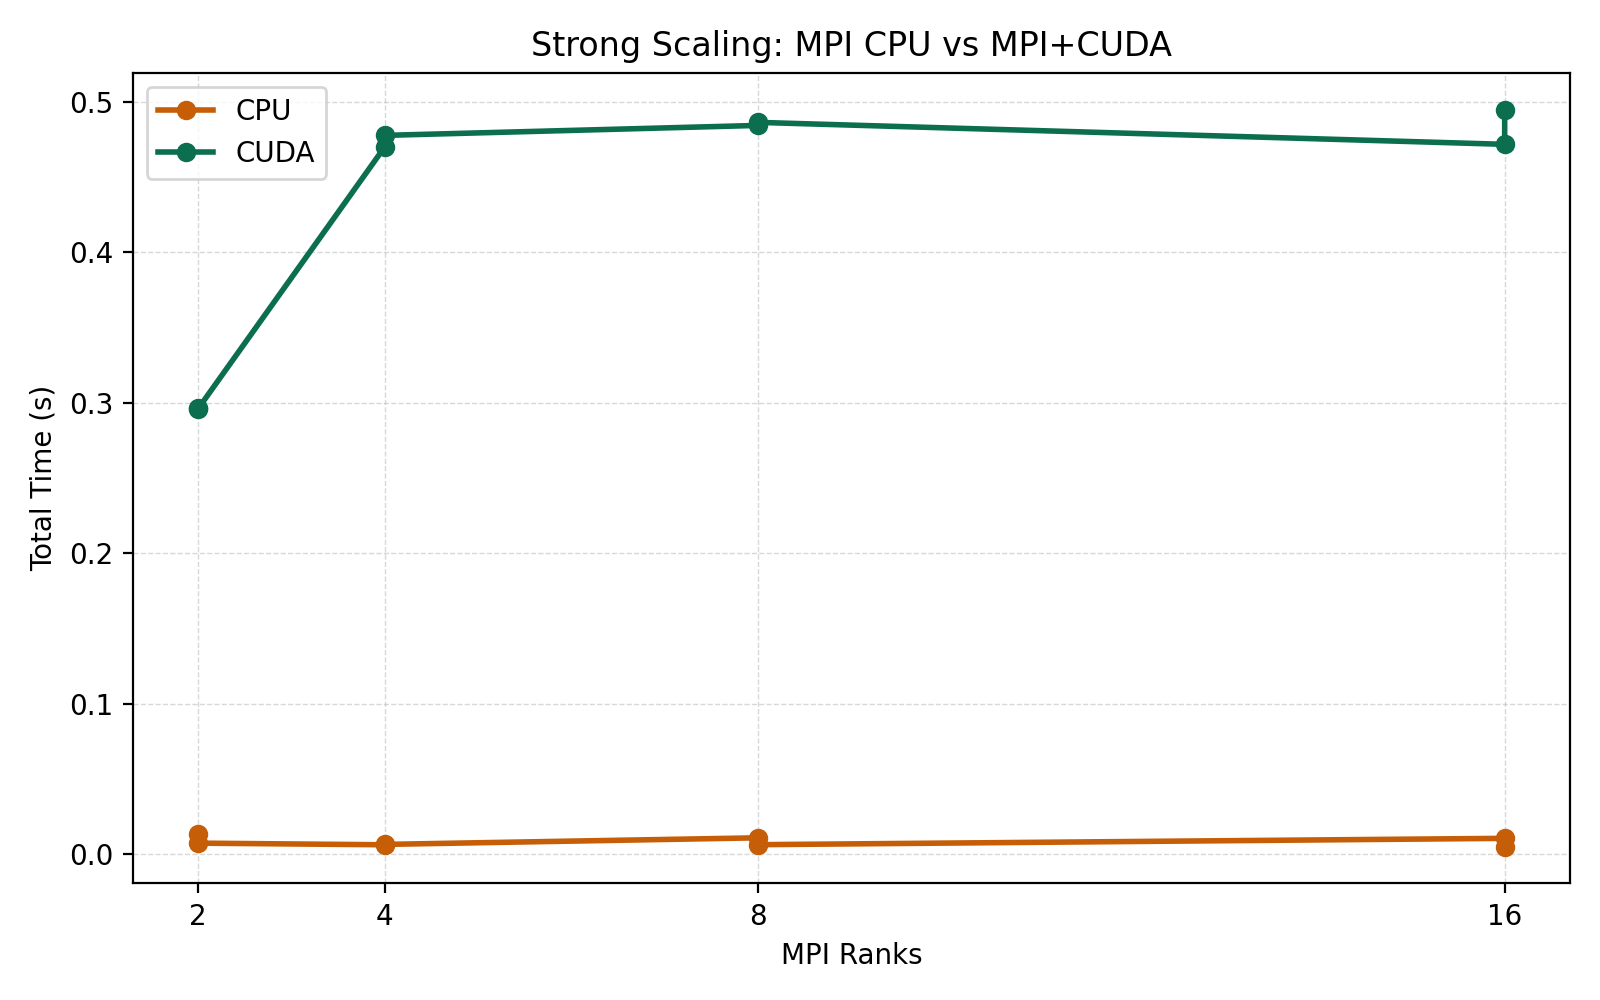
\includegraphics[width=\columnwidth]{strong_scaling_total_time.png}
  \caption{Strong scaling of the CPU-only MPI backend and the hybrid MPI+CUDA backend.}
  \label{fig:strongscaling}
\end{figure}

\begin{figure}[t]
  \centering
  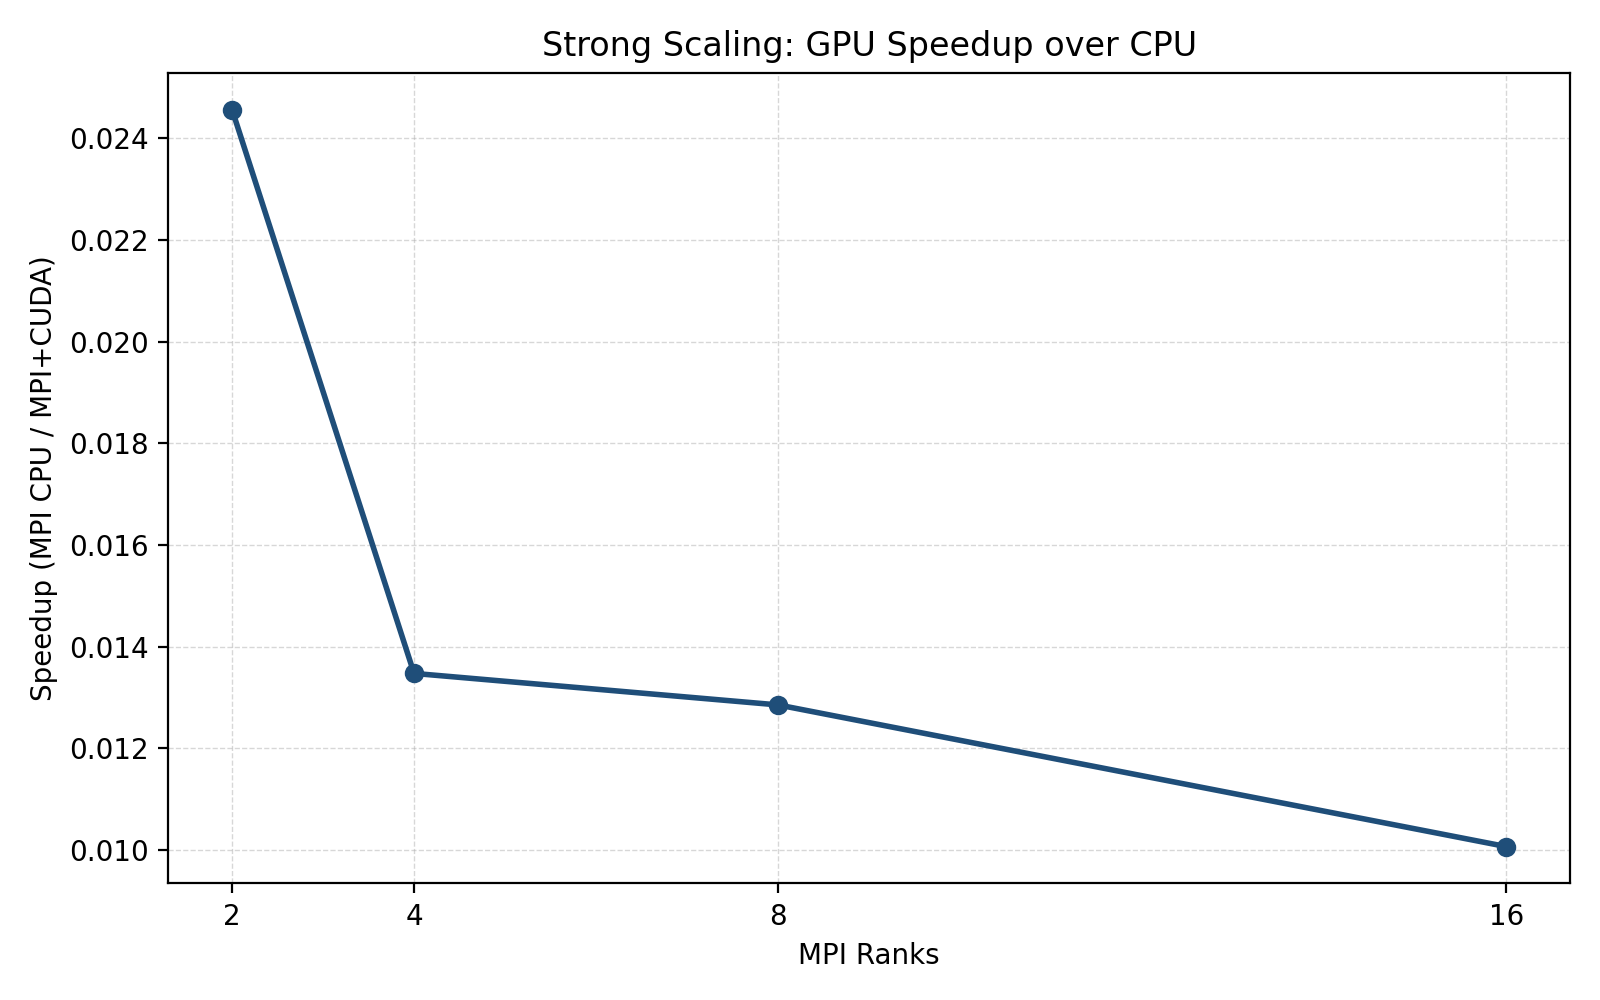
\includegraphics[width=\columnwidth]{strong_gpu_speedup.png}
  \caption{GPU speedup over the CPU-only MPI baseline under strong scaling. Values below 1 indicate that the GPU path is slower end-to-end than the CPU path.}
  \label{fig:strongspeedup}
\end{figure}

\begin{figure}[t]
  \centering
  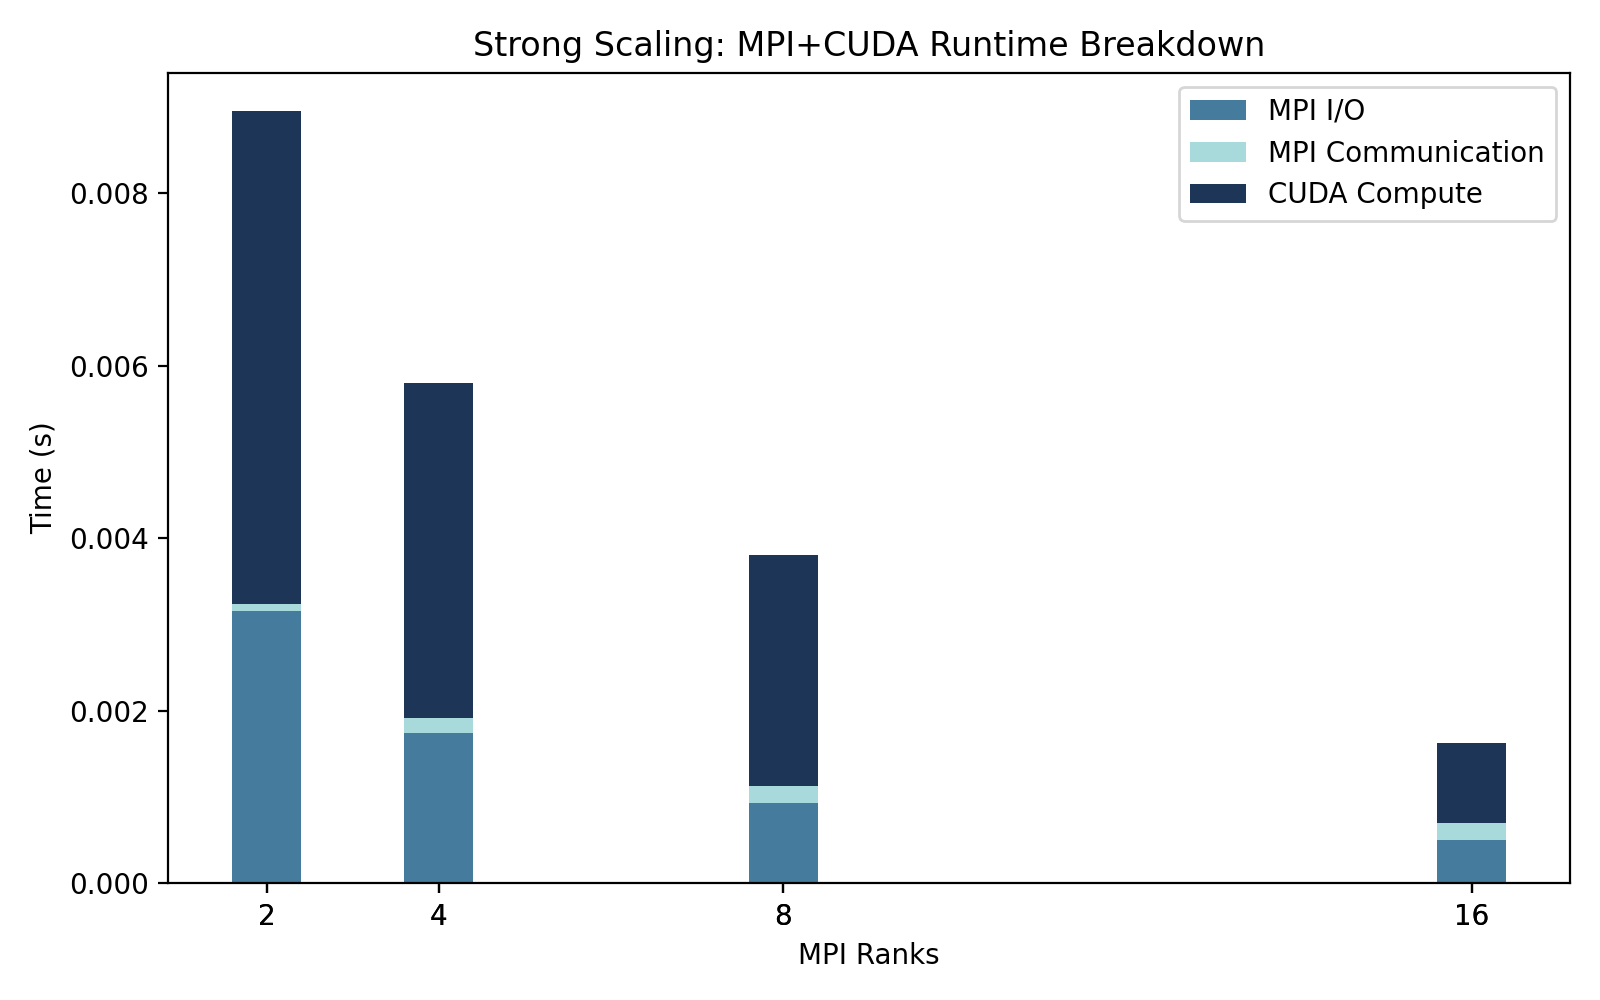
\includegraphics[width=\columnwidth]{strong_cuda_breakdown.png}
  \caption{Strong-scaling runtime breakdown for the hybrid MPI+CUDA backend.}
  \label{fig:strongbreakdown}
\end{figure}

The strong-scaling study fixes the total record count at 400,000 records and increases the number of MPI ranks. The CPU-only MPI backend improves from approximately 7.27 ms at two ranks to 4.98 ms at sixteen ranks, which is modest but directionally correct strong scaling. The CUDA backend behaves differently: while the measured GPU compute time decreases from roughly 5.63 ms to 0.93 ms as ranks increase, the \emph{total} runtime remains near 0.47--0.49 s for 4--16 ranks and is already 0.296 s at two ranks. This means that the GPU kernel itself is not the bottleneck; instead, fixed GPU overhead dominates the full runtime.

This result is visible in Figures~\ref{fig:strongscaling}--\ref{fig:strongbreakdown}. The strong-scaling speedup curve for the GPU path stays well below 1 when compared to CPU-only MPI because total wall-clock time includes CUDA runtime initialization, device setup, host-to-device copies, device-to-host copies, and synchronization. Those costs are not reflected in the explicit \texttt{compute\_seconds} counter alone, so the breakdown figure is essential for interpreting the result correctly. In other words, the GPU accelerates the local analytic kernel but does not yet accelerate the full application.

\section{Weak Scaling Parallel Performance}
\label{sec:weak-scaling}
\begin{figure}[t]
  \centering
  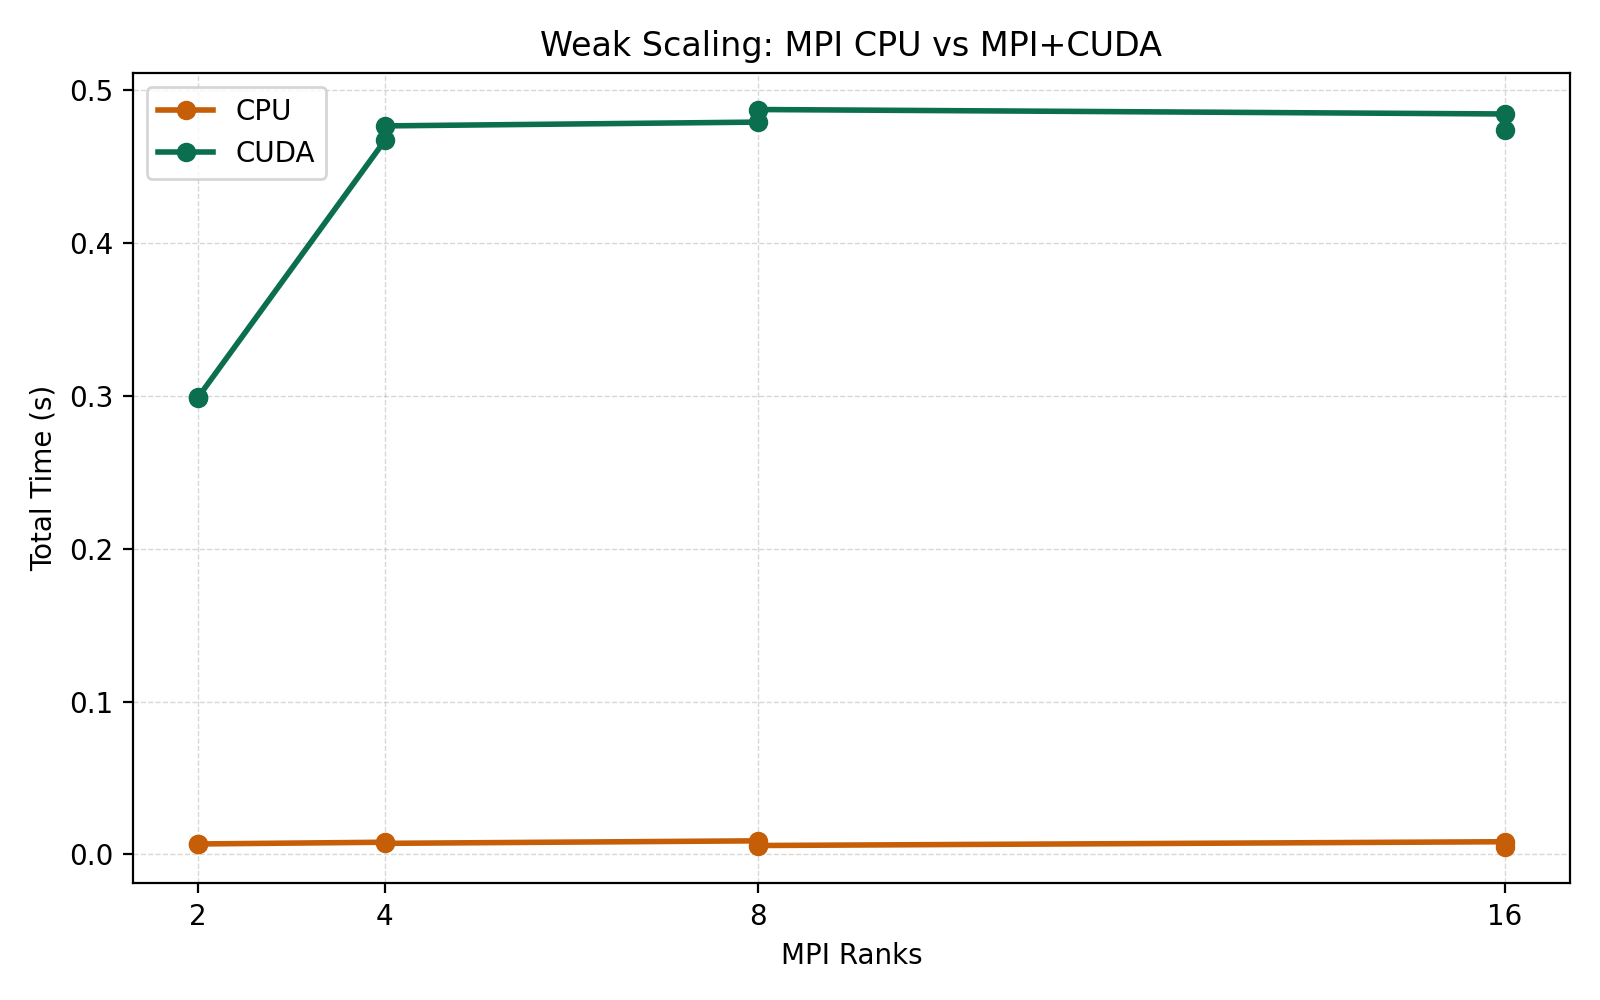
\includegraphics[width=\columnwidth]{weak_scaling_total_time.png}
  \caption{Weak scaling of the CPU-only MPI backend and the hybrid MPI+CUDA backend.}
  \label{fig:weakscaling}
\end{figure}

\begin{figure}[t]
  \centering
  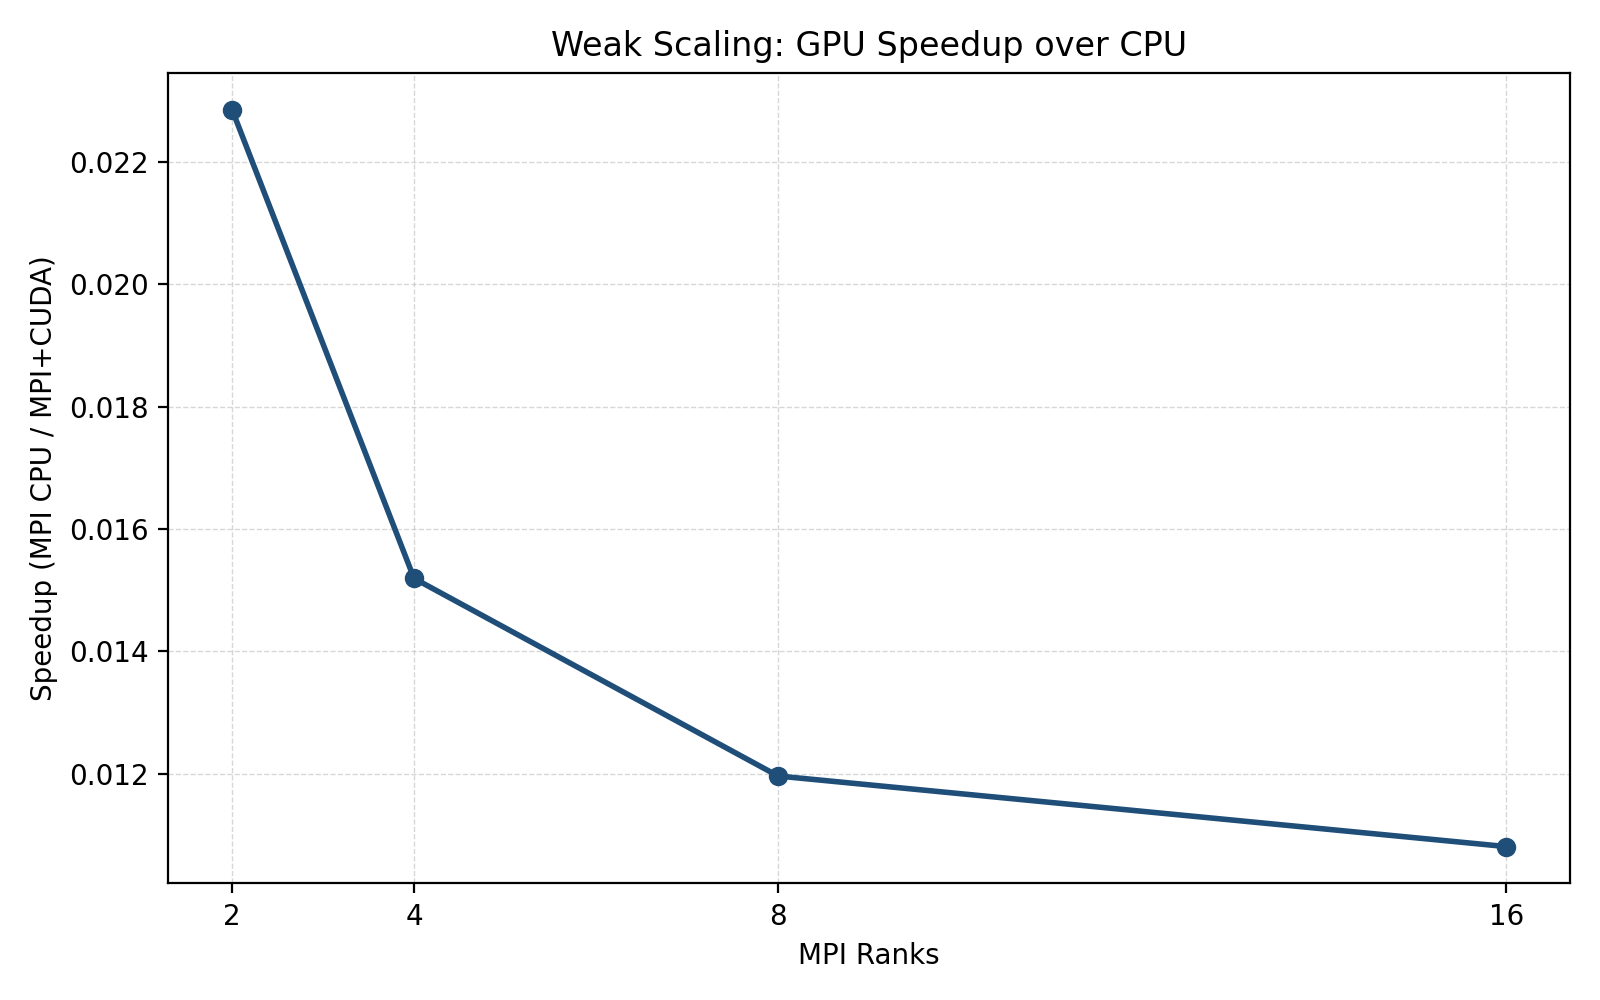
\includegraphics[width=\columnwidth]{weak_gpu_speedup.png}
  \caption{GPU speedup over the CPU-only MPI baseline under weak scaling.}
  \label{fig:weakspeedup}
\end{figure}

\begin{figure}[t]
  \centering
  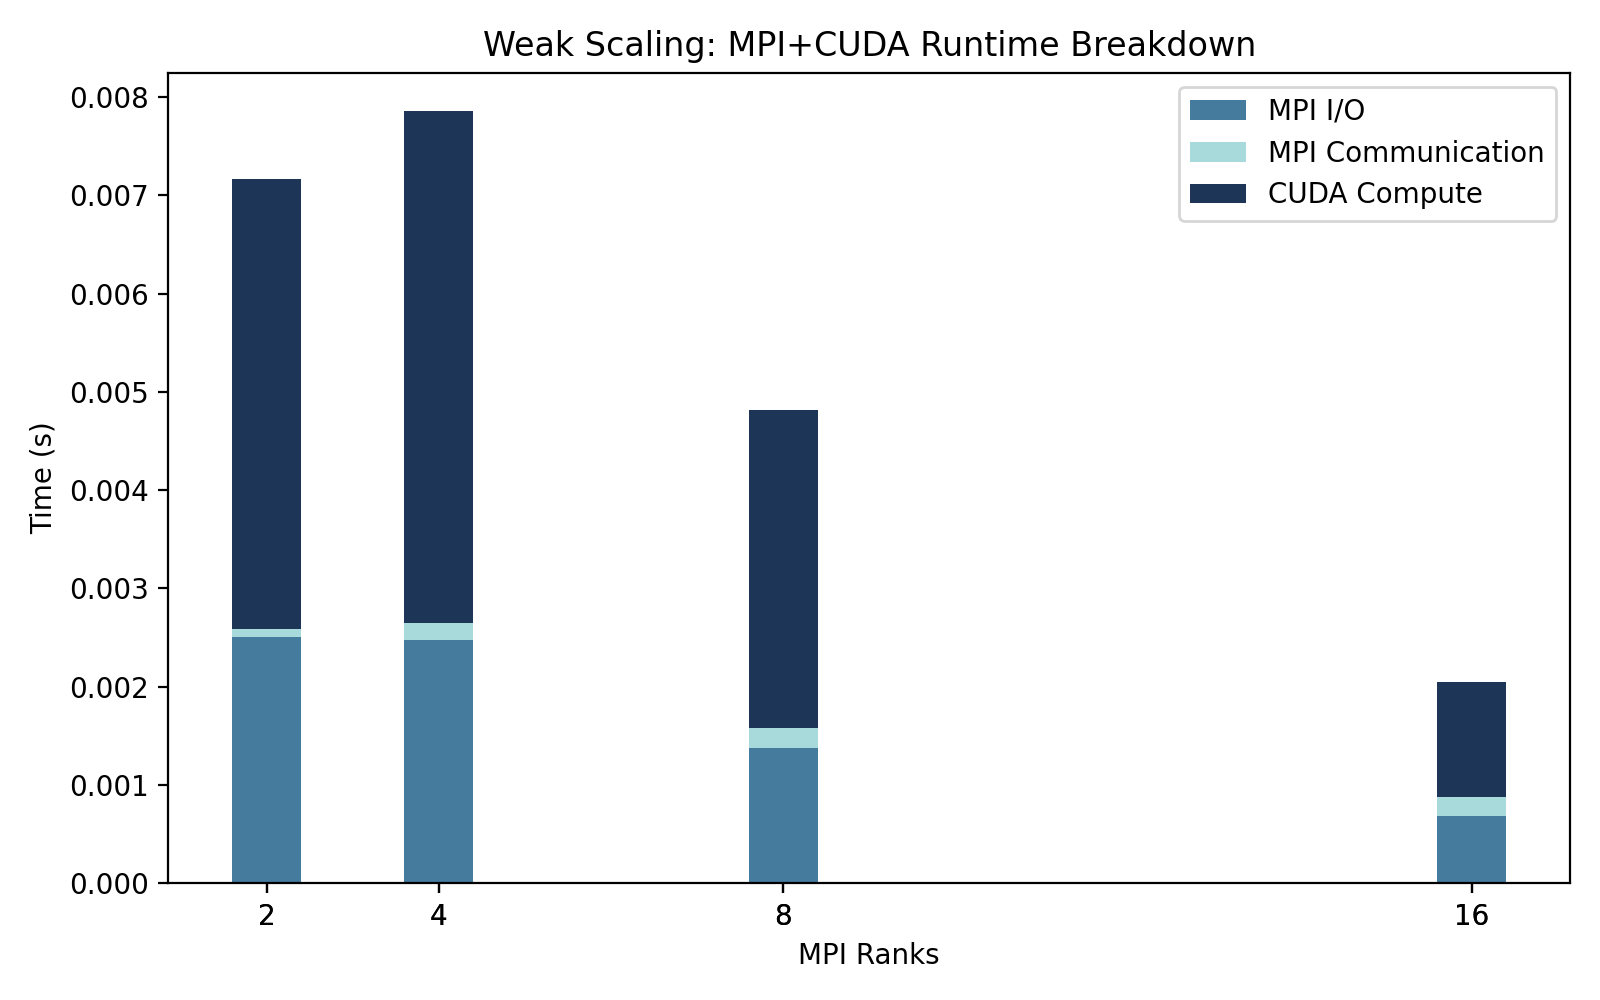
\includegraphics[width=\columnwidth]{weak_cuda_breakdown.png}
  \caption{Weak-scaling runtime breakdown for the hybrid MPI+CUDA backend.}
  \label{fig:weakbreakdown}
\end{figure}

The weak-scaling study fixes the records per rank and increases the total workload with the number of MPI ranks. In the successful runs, the CPU backend remains in a narrow band from 6.84 ms at two ranks to 5.12 ms at sixteen ranks, which is reasonably close to ideal weak scaling given that the total record count grows from 300,000 to the full 576,229 records available in the dataset. The CUDA backend again shows a nearly flat total runtime near 0.47--0.49 s for 4--16 ranks, with a smaller 0.299 s runtime at two ranks. As in strong scaling, the local GPU compute time decreases with more ranks, but the total runtime does not improve because the fixed GPU-side overhead dominates.

The weak-scaling plots therefore reinforce the strong-scaling conclusion: the current implementation demonstrates correct hybrid execution and meaningful GPU-local parallelism, but the application is still overhead-bound in its end-to-end CUDA configuration. That is a legitimate performance result. It shows that simply adding GPU computation to a small or moderate workload does not automatically improve wall-clock time, especially when the local compute phase is short relative to device initialization and memory-transfer costs.

\section{Analysis of Performance Results}
The measured results make the dominant bottlenecks clearer than the original design-level expectations:
\begin{itemize}[leftmargin=*]
  \item \textbf{CUDA runtime overhead dominates total time.} The measured GPU compute phase is only a few milliseconds, but total application time is hundreds of milliseconds, implying that device setup and transfer overhead are the primary bottleneck.
  \item \textbf{MPI-I/O is not the main limiter in these runs.} The measured I/O times are on the order of 0.5--3.2 ms, which is small relative to GPU total runtime and comparable to or slightly larger than the CPU local compute phase.
  \item \textbf{Boundary exchange and reduction are negligible at current scale.} Both remain in the microsecond range, so they do not dominate either backend in the present dataset size.
  \item \textbf{The CPU baseline is strong because the local workload is modest.} With at most 576,229 records total, the host-side loops are inexpensive enough that GPU acceleration cannot amortize its fixed costs.
\end{itemize}

The main performance lesson is therefore architectural rather than purely numerical. A hybrid MPI+CUDA design is not automatically faster than MPI on CPUs; it becomes faster only when the local compute intensity is high enough to amortize the GPU’s fixed runtime costs. In the current implementation, that threshold has not yet been reached for the chosen workload sizes, so the GPU path is slower in total runtime even though its measured local kernel work scales sensibly. This is exactly the kind of communication-versus-computation explanation the assignment asks for.

\section{Discussion}
The provider-level analytics already show why this application is worth parallelizing. The consolidated dataset is large enough to be annoying in raw GTFS form, and even the fixed-width representation still contains more than half a million trip records across multiple systems. The New York provider grouping alone contributes nearly 300,000 trips and several distinct operating modes. Such a dataset is manageable for one local pass, but the moment one wants repeated parameter sweeps, additional providers, or the integration of GTFS-Realtime, the need for scalable ingestion and analysis becomes much clearer.

The current provider findings are also useful in their own right. NJ Transit appears the most peak-concentrated and the most headway-sparse among the provider groups studied here, which matches intuition about a commuter-oriented system. CTA and MTA exhibit the shortest route-level median headways, consistent with dense urban service. MBTA’s mode mix is richer than CTA’s and includes ferry routes, while SEPTA sits between MBTA and NJ Transit in median route headway. These are schedule-based findings, not passenger-based conclusions, but they provide a meaningful cross-city operational picture.

One practical lesson from the data-engineering stage is that publicly available GTFS feeds are cleaner in schema than in packaging. Missing \texttt{calendar.txt} files, nested archives, and extended route-type codes all had to be handled explicitly before the HPC work could even begin. This preprocessing burden is easy to overlook in abstract algorithm descriptions, but it is central to building a publishable system around real data.

Another lesson is that schedule analytics become much more interesting when multiple metrics are placed next to one another instead of interpreted in isolation. Peak/off-peak ratios alone make the agencies look somewhat similar, but route intensity, service span, and duration distributions separate them more clearly. MTA and CTA are both high-intensity systems by trips per route, yet MTA sustains that intensity across a longer service-day span. MBTA has a broader mode mix and a shorter median trip duration than the commuter-oriented providers. NJ Transit’s strong peak concentration becomes more meaningful once it is paired with its longer durations, larger headways, lower route intensity, and higher wide-gap rate. These cross-metric comparisons make the provider study read more like a systems paper and less like a single-metric benchmark.

\section{Team Contributions}
Replace this section with the actual team roster and contribution details. A concise format that satisfies the rubric is one paragraph per member:
\begin{itemize}[leftmargin=*]
  \item \textbf{Member A}: implemented preprocessing and dataset construction, handled GTFS packaging edge cases, and validated provider summaries.
  \item \textbf{Member B}: implemented MPI partitioning, MPI-I/O, and global reduction logic.
  \item \textbf{Member C}: implemented CUDA kernels, device-memory management, and CPU-versus-GPU comparison support.
  \item \textbf{Member D}: executed AiMOS experiments, collected timing data, generated figures, and integrated the report narrative and references.
\end{itemize}

\section{Conclusions and Future Work}
This project demonstrates that GTFS schedule feeds can be transformed into a meaningful massively parallel analytics workload using MPI, MPI-I/O, and CUDA. The binary trip-record representation makes collective shared-file access practical, the boundary-exchange step prevents the workload from collapsing into embarrassingly parallel map-only processing, and the CUDA path provides a natural hybrid baseline against CPU-only MPI execution. The provider-side results reveal meaningful differences in peak concentration, route headways, service span, trip duration, route intensity, and mode composition across MTA, CTA, MBTA, NJ Transit, and SEPTA.

The completed AiMOS timing study also produced a result that is technically valuable even though it was not the naive best-case outcome. The MPI+CUDA path runs correctly and its local kernel time scales in the expected direction, but the full application remains slower than CPU-only MPI because the problem size is still too small to amortize GPU initialization and transfer overhead. That finding is exactly the kind of end-to-end explanation that a hybrid HPC paper should include: not just whether acceleration exists in principle, but where it is lost in the actual pipeline.

Beyond the current prototype, the most promising extensions are:
\begin{itemize}[leftmargin=*]
  \item integrating \texttt{calendar\_dates.txt} exceptions more explicitly,
  \item expanding \texttt{frequencies.txt} into generated trips when needed,
  \item adding GTFS-Realtime delay records to support true reliability analysis,
  \item experimenting with NVMe staging versus direct shared-file access, and
  \item extending the workload to more cities and longer time horizons.
\end{itemize}

With those additions, the project could evolve from a schedule-analytics case study into a richer real-time transit-performance platform while retaining its value as a nontrivial hybrid HPC application.

\bibliographystyle{ACM-Reference-Format}
\bibliography{references}

\end{document}
